\documentclass[a4paper,12pt]{article}

\usepackage[utf8]{inputenc}
\usepackage[czech]{babel}
\usepackage[IL2]{fontenc}
\usepackage[left=3cm,text={15cm, 23cm},top=3.5cm]{geometry}

\usepackage{graphicx}
\usepackage{tikz}

\usepackage{amssymb}
\usepackage{amsmath}
\usepackage{amsthm}
\usepackage{forest}
\usepackage[ruled,czech,linesnumbered,noline]{algorithm2e}
\usepackage{array}
\usepackage{multirow}
\usepackage{textcomp}
\usepackage{listings}

\usepackage{enumitem}

\usepackage{pgf}
\usepackage{tikz}
\usetikzlibrary{arrows,automata}

\newcounter{counten}
\setcounter{counten}{1}


\title{\bf PRL Projekt 2\,--\,Enumeration sort}
\author{Vojtěch Havlena (xhavle03)}
\date{\today}

\begin{document}

\maketitle


\section{Rozbor a analýza algoritmu}
Algoritmus Enumeration sort využívá lineární spojení $n$ procesorů, které je doplněno o společnou 
sběrnici. Vstupem je posloupnost čísel $(x_1, \dots, x_n)$. Každý procesor $i$ má k dispozici registry 
$X_i$, $Y_i$, $Z_i$ a $C_i$. Samotný algoritmus lze potom popsat následujícími kroky:
\begin{enumerate}[noitemsep]
 \item Každý procesor $i$ si nastaví hodnotu registru $C_i$ na 1.
 \item Následující kroky se v cyklu pro $1\leq k \leq 2n$ opakují $2n$ krát:
 \begin{enumerate}[noitemsep,label=(\alph*)]
  \item V případě, že postupně zpracovávaná vstupní posloupnost ještě není vyčerpána (tj. $k \leq n$), 
  prvek $x_k$ se (sběrnicí) vloží do registru $X_k$, obsah registrů $Y$ všech procesorů se posune 
  doprava (lineárním spojením) a do registru $Y_1$ se (lineárním spojením) vloží $x_k$. 
  \item Každý procesor, který má již v registrech $X$ a $Y$ uložené hodnoty ze vstupu, provede 
  porovnání těchto hodnot. Je-li $X > Y$, inkrementuje obsah registru $C$.
  \item Po vyčerpání vstupní posloupnosti (tj. $k > n$) procesor $P_{k-n}$ pošle obsah svého registru 
  $X$ procesoru $P_{C_{k-n}}$, který si tuto hodnotu uloží do svého registru $Z$.
 \end{enumerate}
 \item V dalších $n$ cyklech jednotlivé procesory postupně posouvají obsah svých registrů $Z$ směrem 
 doprava a procesor $P_n$ produkuje výslednou seřazenou posloupnost.
\end{enumerate}

\subsection*{Analýza složitosti}
V prvním kroku algoritmu si paralelně všechny procesory nastaví hodnotu registru $C$ na 1. Časová složitost 
tohoto kroku je tedy $\mathcal{O}(1)$. Kroky 2a, 2b a 2c provádí porovnání a poslání konstantního 
počtu hodnot. Tedy časová složitost těchto kroků je rovněž $\mathcal{O}(1)$. Provádění těchto kroků 
je opakováno celkem $2n$ krát. Celková časová složitost kroku 2 je tedy $\mathcal{O}(n)$. Posuv hodnoty v 3. 
kroku lze provést v konstantním čase a tento posuv se provádí v cyklu $n$ krát. Časová složitost kroku 
3 je tedy $\mathcal{O}(n)$. Celkovou časovou složitost algoritmu lze vyjádřit jako
\begin{equation}
  t(n) = \mathcal{O}(1) + \mathcal{O}(n) + \mathcal{O}(n) = \mathcal{O}(n).
\end{equation}
Vzhledem k tomu, že algoritmus pracuje na lineárním poli $n$ procesorů, počet procesorů 
je $p(n) = n$. Celková cena je tedy
\begin{equation}
  c(n) = p(n)\cdot t(n) = \mathcal{O}(n^2).
\end{equation}

\section{Implementace}
Algoritmus byl implementován v jazyce C++ s využitím knihovny Open MPI. Implementace pro seřazení $n$ hodnot 
využívá $n+1$ procesorů. Procesory jsou označeny jednoznačnými číselnými identifikátory z $\{0,\dots,n\}$ 
(Rank). Procesory jsou pomocí svých hodnot Rank označeny jako $P_0, \dots, P_n$ Procesor s $P_0$ (master) se na samotném řazení 
nepodílí, pouze posílá načtené hodnoty jednotlivým procesorům a na konci získává seřazenou posloupnost.

Pro správné odlišení zpráv je využíváno značení zpráv MPI pomocí položky TAG. Zprávy, které posílá master procesoru $P_i$ pro 
uložení vstupní hodnoty $x_i$ do registru $X_i$, jsou označeny \texttt{TAG\_BUS}. 
Hlavní cyklus posouvání prvků vstupní posloupnosti a jejich porovnávání s aktuální hodnotou $X$ probíhá v 
$n$ krocích. Postupné posouvání vstupních hodnot mezi sousedními procesory ($P_i$ a $P_{i+1}$) je umožněno 
zprávami, které jsou označeny \texttt{TAG\_INPUT}. Po porovnání všemi vstupními hodnotami, procesor $P_i$
pošle obsah $X_i$ procesoru $P_{C_i}$ pomocí zprávy označené jako \texttt{TAG\_RESULT\_INTER}. Nakonec je 
obsah registrů $Z$ posouván pomocí zpráv označených \texttt{TAG\_RESULT\_OUT}.

Algoritmus byl rovněž upraven, aby byl schopen řadit posloupnosti obsahující stejná čísla. Hodnota $C$
je inkrementována pokud $X > Y$ nebo v případě, že $X \geq Y$, ale to jen pokud pořadí prvku vstupní 
posloupnosti, který je uložen v $Y$, je menší než Rank procesoru.

\section{Komunikační protokol}
Jak již bylo popsáno v sekci Implementace, pro rozlišení zpráv se používá jejich značení (TAG). Komu se má 
zaslat zpráva záleží na hodnotě Rank procesoru. 
Na začátku algoritmu, procesor $P_0$ (master) posílá jednotlivé 
vstupní hodnoty $x_k$ procesorům $P_1$ a $P_k$, kde $1 \leq k \leq n$. Dále každý procesor $P_i$, kde 
$1 \leq i \leq n-1$ postupně posílá hodnotu $Y$ svému pravému sousedovi (procesoru $P_{i+1}$). Až procesor 
$P_i$ provede porovnání se všemi vstupními hodnotami, posílá zprávu procesoru $P_{C_i}$. Poté, co všechny 
procesy (kromě $P_0$) obdrží hodnotu, každý procesor $P_i$ postupně posílá hodnoty $Z_i$ procesoru $P_{i+1}$ 
($P_n$ posílá hodnoty procesoru $P_0$). Komunikační protokol je vizualizován na obrázku~\ref{fig:seq} (pro 
přehlednost je umístěn na poslední straně).

\section{Experimenty}
Cílem experimentů je ověřit, zda teoreticky odvozená časová složitost odpovídá reálné časové složitosti 
(době provádění algoritmu). Doba provádění algoritmu je měřena pomocí funkce \texttt{MPI\_Wtime}. Do doby 
provádění algoritmu není započítáno načítání vstupní posloupnosti a výpis seřazené posloupnosti na výstup. 
Doba provádění se začíná měřit až v okamžiku, kdy jsou všechny procesory připraveny zahájit řazení (toho 
je docíleno pomocí bariéry). Měření končí, když procesor s $P_0$ (master) obdrží seřazenou posloupnost. 

Experimenty byly provedeny pro velikosti vstupu 5\,--\,30 hodnot. Měření probíhalo na lokálním stroji 
(Debian, Intel Core i5) a na serveru Merlin. Měření pro každou velikost vstupu bylo 
provedeno celkem 50 krát a tyto hodnoty byly zprůměrovány. Výsledky experimentů jsou uvedeny na obrázku~\ref{fig:exp}.

\begin{figure}[h]
  \centering
  \includegraphics{Figures/merge-res.eps}
  \caption{Výsledky provedených experimentů.}
  \label{fig:exp}
\end{figure}

\section{Závěr}
Cílem projektu bylo implementovat algoritmus Enumeration sort a ověřit, zda skutečná doba provádění 
odpovídá teoretické časové složitosti. Z 
experimentů vyplynulo, že pro menší počty vstupních hodnot (cca do 25) je průběh opravdu lineární, 
což odpovídá teoretické časové složitosti. Pro větší počet vstupních hodnot již dochází k odchýlení 
od lineárního průběhu. Navíc pro tyto vyšší hodnoty je i větší rozptyl naměřených časů. Odchylka může být 
způsobena režií posílání zpráv, přepínáním procesů nebo také aktuálním vytížením procesorů 
(časová složitost by měla být lineární v případě, že procesy poběží skutečně paralelně, což minimálně 
na lokálním stroji splněno nebylo).

\begin{figure}
  \centering
  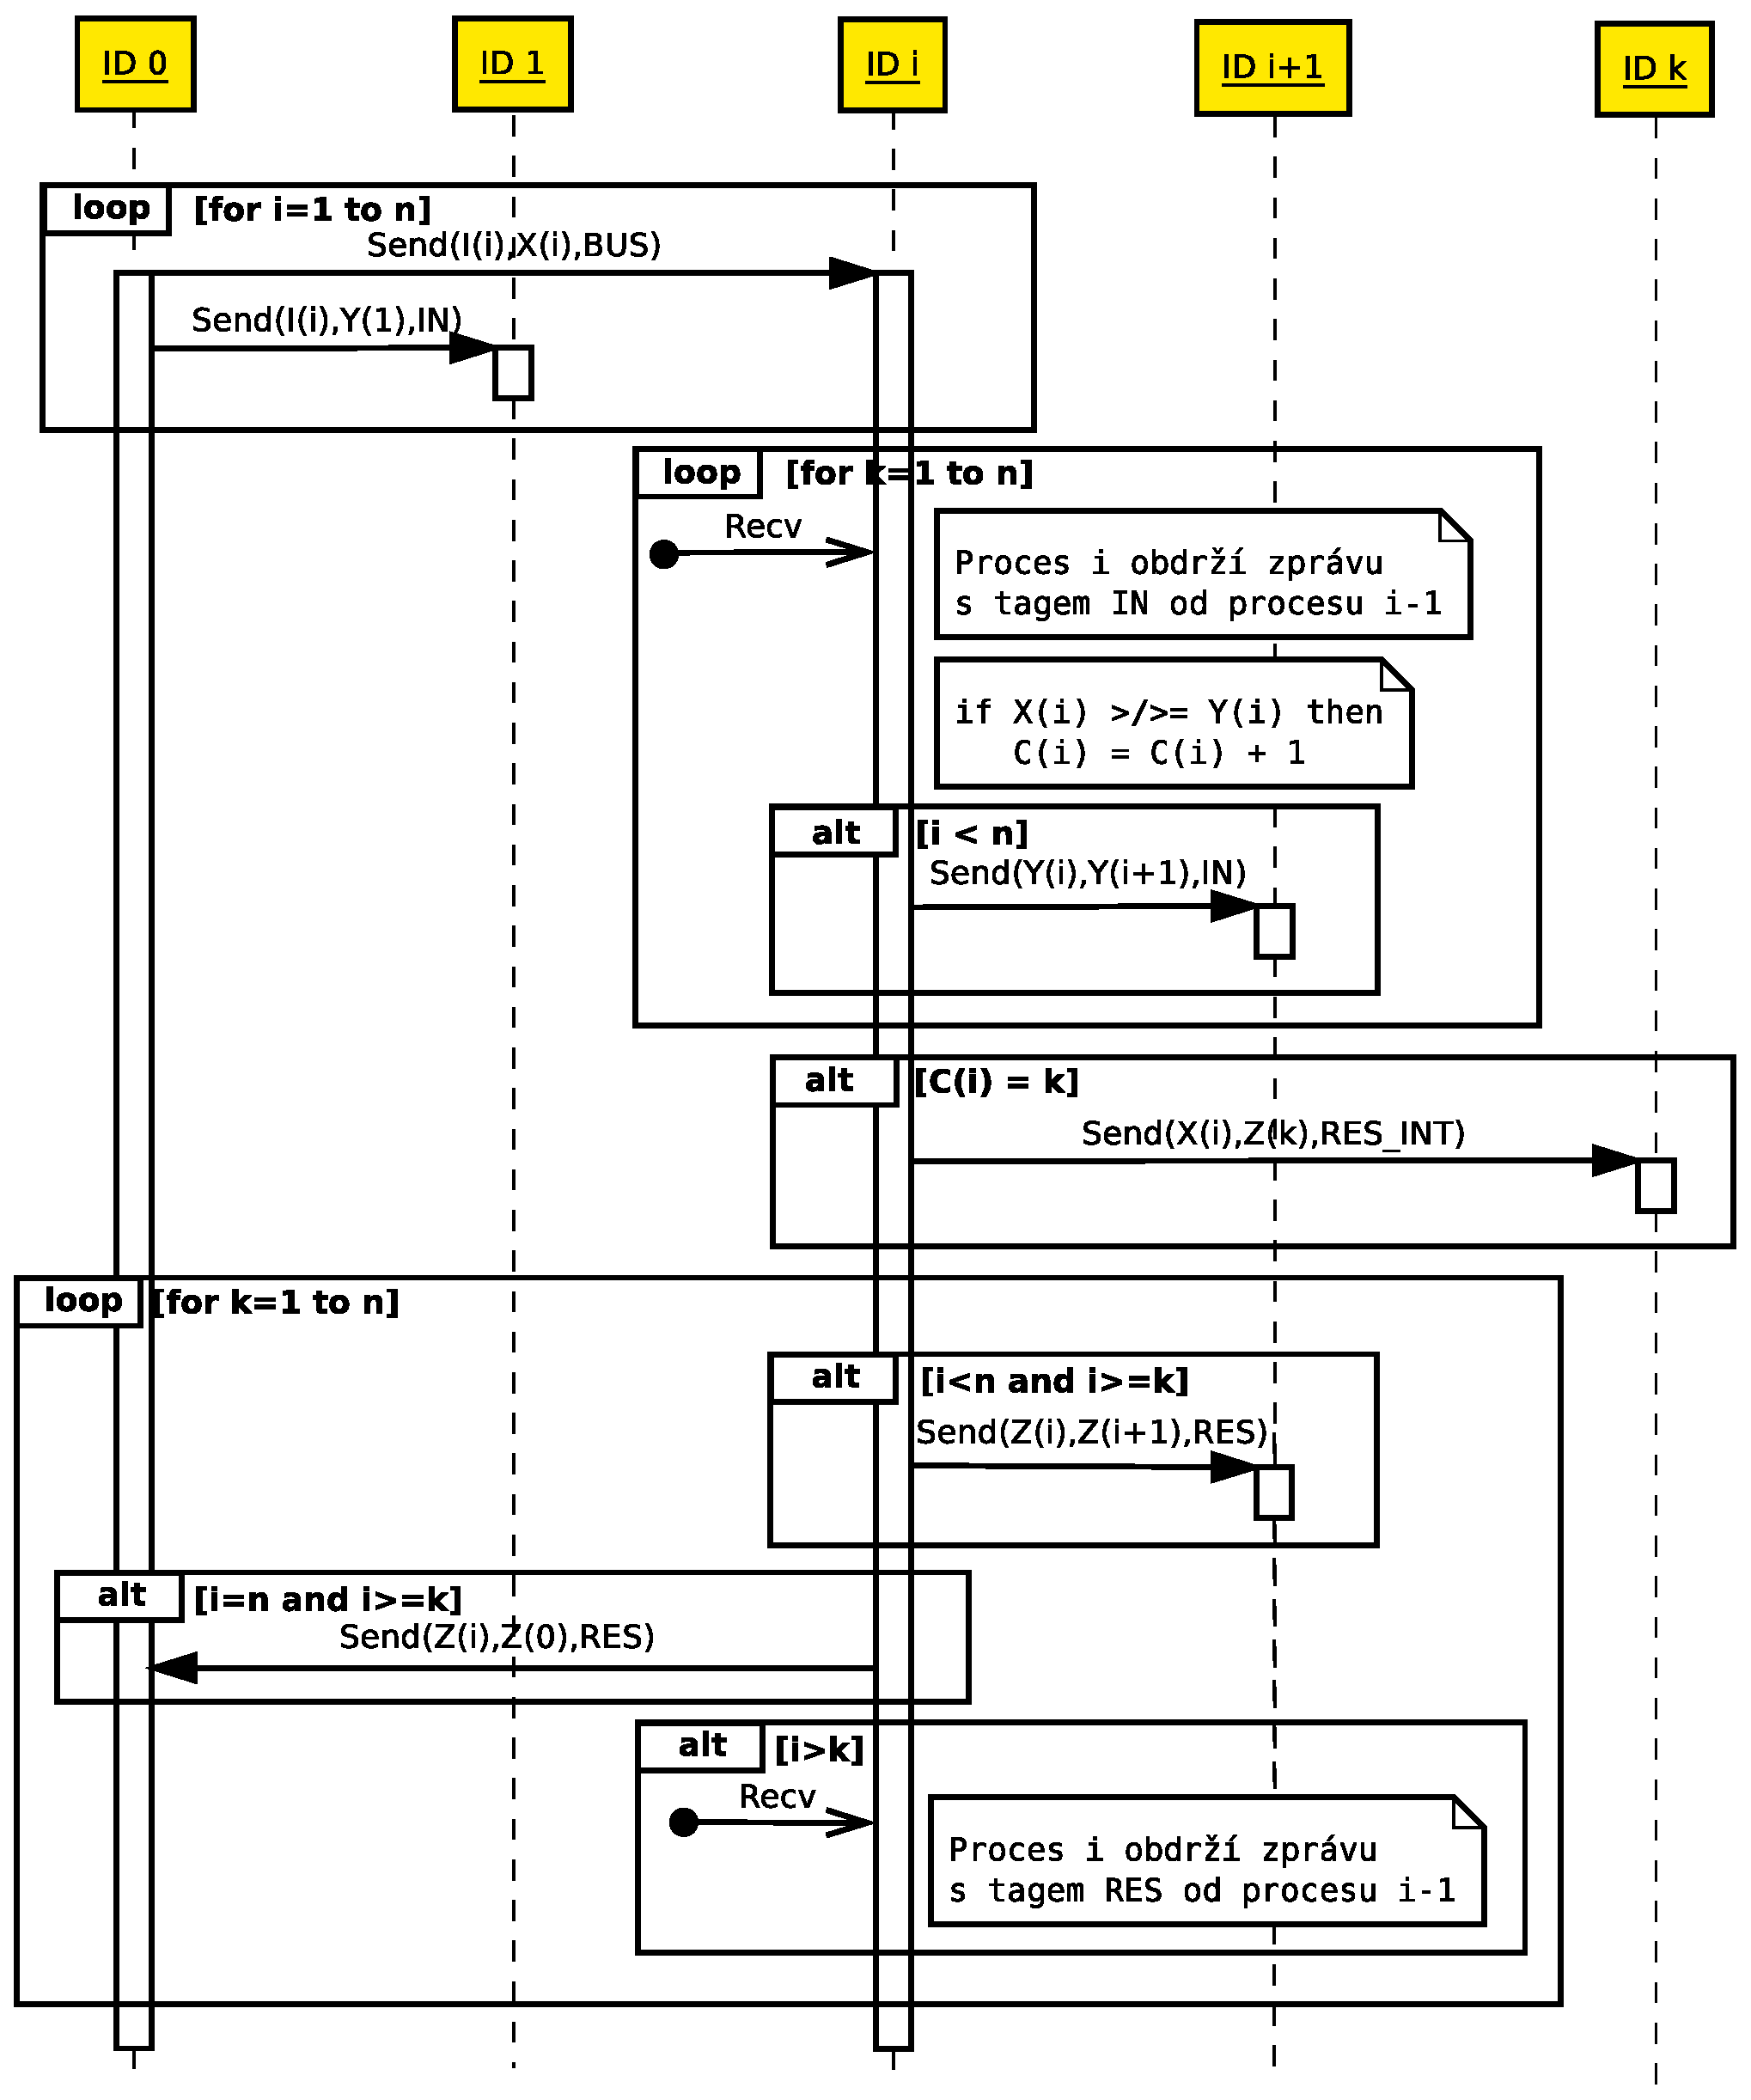
\includegraphics[scale=0.3]{Figures/SequenceDiagramCompress.eps}
  \caption{Komunikační protokol pro $n$ procesorů. Procesory jsou rozlišeny pomocí hodnoty Rank. Zasílání zpráv je 
  označeno plnou šipkou s popisem Send($Odkud$, $Kam$, $Tag$), kde $Odkud$ je posílaná hodnota, $Kam$ je místo uložení 
  a $Tag$ je zkratka označení zprávy (jednotlivá označení jsou popsána v sekci Implementace). Pomocí šipky s kulatým koncem s nápisem Recv je 
  znázorněno přijetí zprávy (zpráva byla odeslána již dříve). Prvek na pozici $i$ vstupní neseřazené 
  posloupnosti je označen jako $I(i)$.}
  \label{fig:seq}
\end{figure}

\end{document}	
